\documentclass{beamer}

\usefonttheme{professionalfonts} % using non standard fonts for beamer
\usefonttheme{serif} % default family is serif

%\usepackage{hyperref}

%\usepackage{minted}

\usepackage{animate}

\usepackage{graphicx}

\def\Put(#1,#2)#3{\leavevmode\makebox(0,0){\put(#1,#2){#3}}}

\usepackage{color}

\usepackage{tikz}

\usepackage{amssymb}

\usepackage{enumerate}


\newcommand\blfootnote[1]{%

  \begingroup

  \renewcommand\thefootnote{}\footnote{#1}%

  \addtocounter{footnote}{-1}%

  \endgroup

}

\makeatletter

%%%%%%%%%%%%%%%%%%%%%%%%%%%%%% Textclass specific LaTeX commands.

 % this default might be overridden by plain title style

 \newcommand\makebeamertitle{\frame{\maketitle}}%

 % (ERT) argument for the TOC

 \AtBeginDocument{%

   \let\origtableofcontents=\tableofcontents

   \def\tableofcontents{\@ifnextchar[{\origtableofcontents}{\gobbletableofcontents}}

   \def\gobbletableofcontents#1{\origtableofcontents}

 }

%%%%%%%%%%%%%%%%%%%%%%%%%%%%%% User specified LaTeX commands.

\usetheme{Malmoe}

% or ...

\useoutertheme{infolines}

\addtobeamertemplate{headline}{}{\vskip2pt}



\setbeamercovered{transparent}

% or whatever (possibly just delete it)

\makeatother

\begin{document}
\title[DDCEL report]{A Scalable DCEL implementation}
\author[AC]{Andres Calderon}
\institute[Spring'20]{University of California, Riverside}
\makebeamertitle
\newif\iflattersubsect

\AtBeginSection[] {
  \begin{frame}<beamer>
    \frametitle{Outline} 
    \tableofcontents[currentsection]  
  \end{frame}
  \lattersubsectfalse
}

\AtBeginSubsection[] {
  \begin{frame}<beamer>
    \frametitle{Outline} 
    \tableofcontents[currentsubsection]  
  \end{frame}
}

\begin{frame}{A Scalable DCEL...}{Local DCELs}
    \centering
	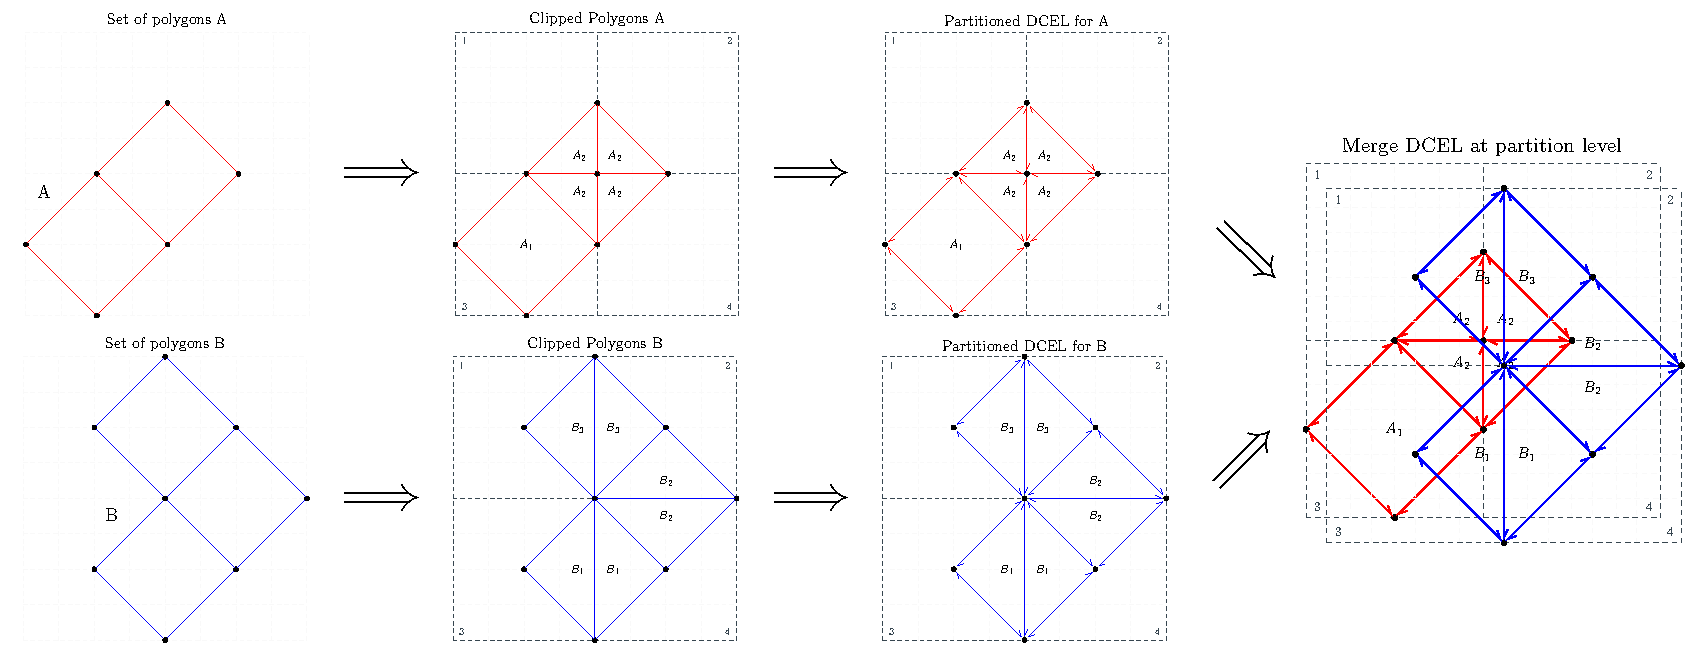
\includegraphics[width=1\textwidth]{figures/01-MergeSteps/OverlayParted}
\end{frame}

\begin{frame}{A Scalable DCEL...}{Merged DCEL}
    \centering
	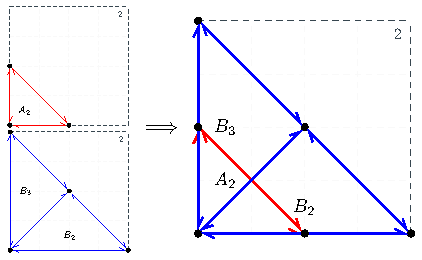
\includegraphics[width=1\textwidth]{figures/02-Splits/Part2}
\end{frame}
\begin{frame}{A Scalable DCEL...}{Merged DCEL}
    \centering
	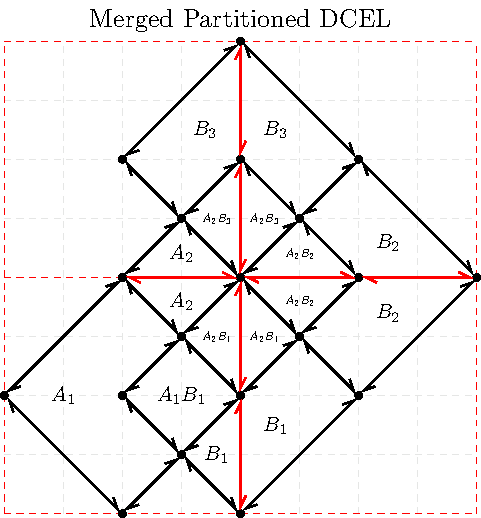
\includegraphics[trim=0 0 0 6mm, clip,width=0.55\textwidth]{figures/03-Overlays1/FinalPartitionedDCEL}
\end{frame}

\begin{frame}{A Scalable DCEL...}{Overlay Operations}
    \centering
	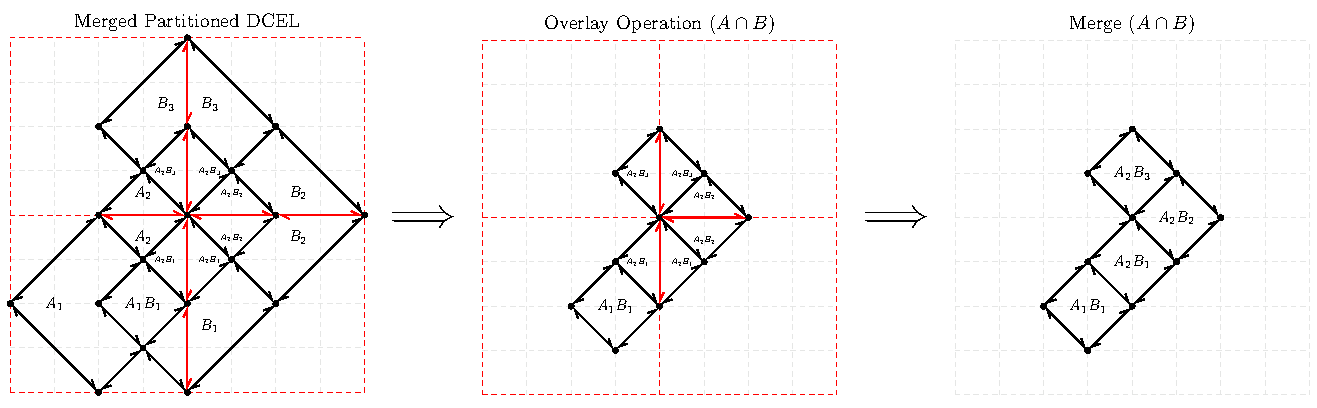
\includegraphics[width=1\textwidth]{figures/03-Overlays1/OverlayParted2}
\end{frame}

\begin{frame}{A Scalable DCEL...}{Overlay Operations}
    \centering
	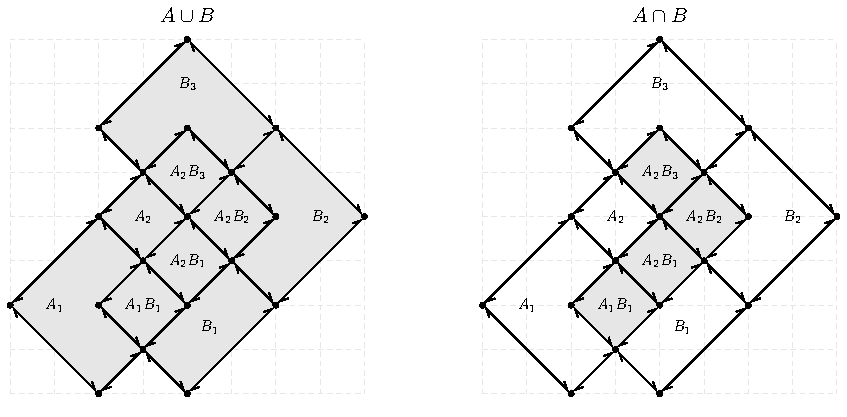
\includegraphics[width=1\textwidth]{figures/04-Overlays2/OverlayOperations1}
\end{frame}
\begin{frame}{A Scalable DCEL...}{Overlay Operations}
    \centering
	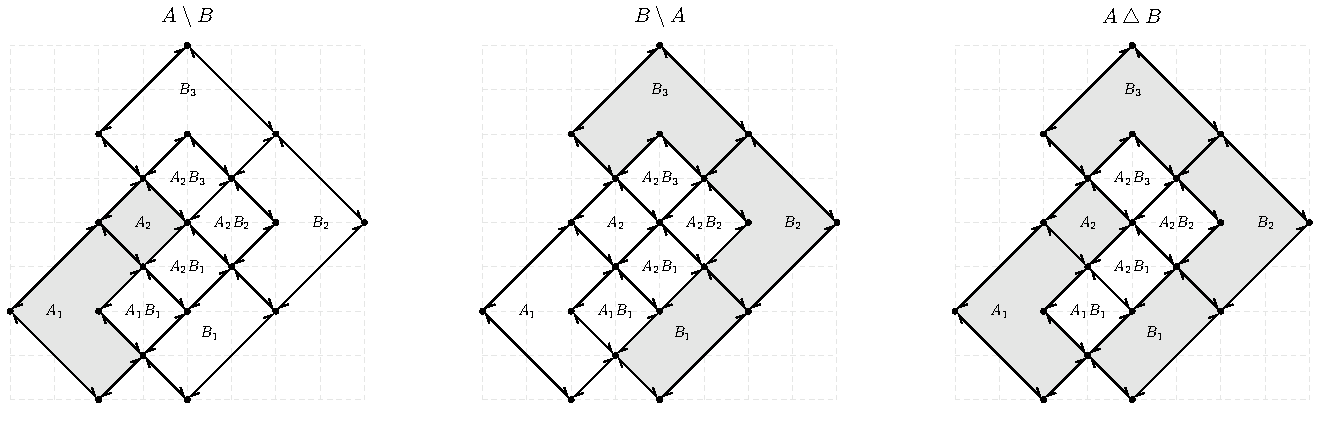
\includegraphics[width=1\textwidth]{figures/04-Overlays2/OverlayOperations2}
\end{frame}

\begin{frame}{The Empty Cell problem...}
    \centering
	\includegraphics[page=4,width=0.6\textwidth]{figures/05-EmptyCells/Example}
\end{frame}
\begin{frame}{The Empty Cell problem...}
    \begin{enumerate}
        \item Identify the quadrant father $Q$ of the current empty cell.
        \item Find the other 3 cells whose touch the center of $Q$.
        \item If one of them has edges: You are done.
        \item If not: choose one of them and repeate.
    \end{enumerate}
\end{frame}
\begin{frame}{The Empty Cell problem...}
    \centering
	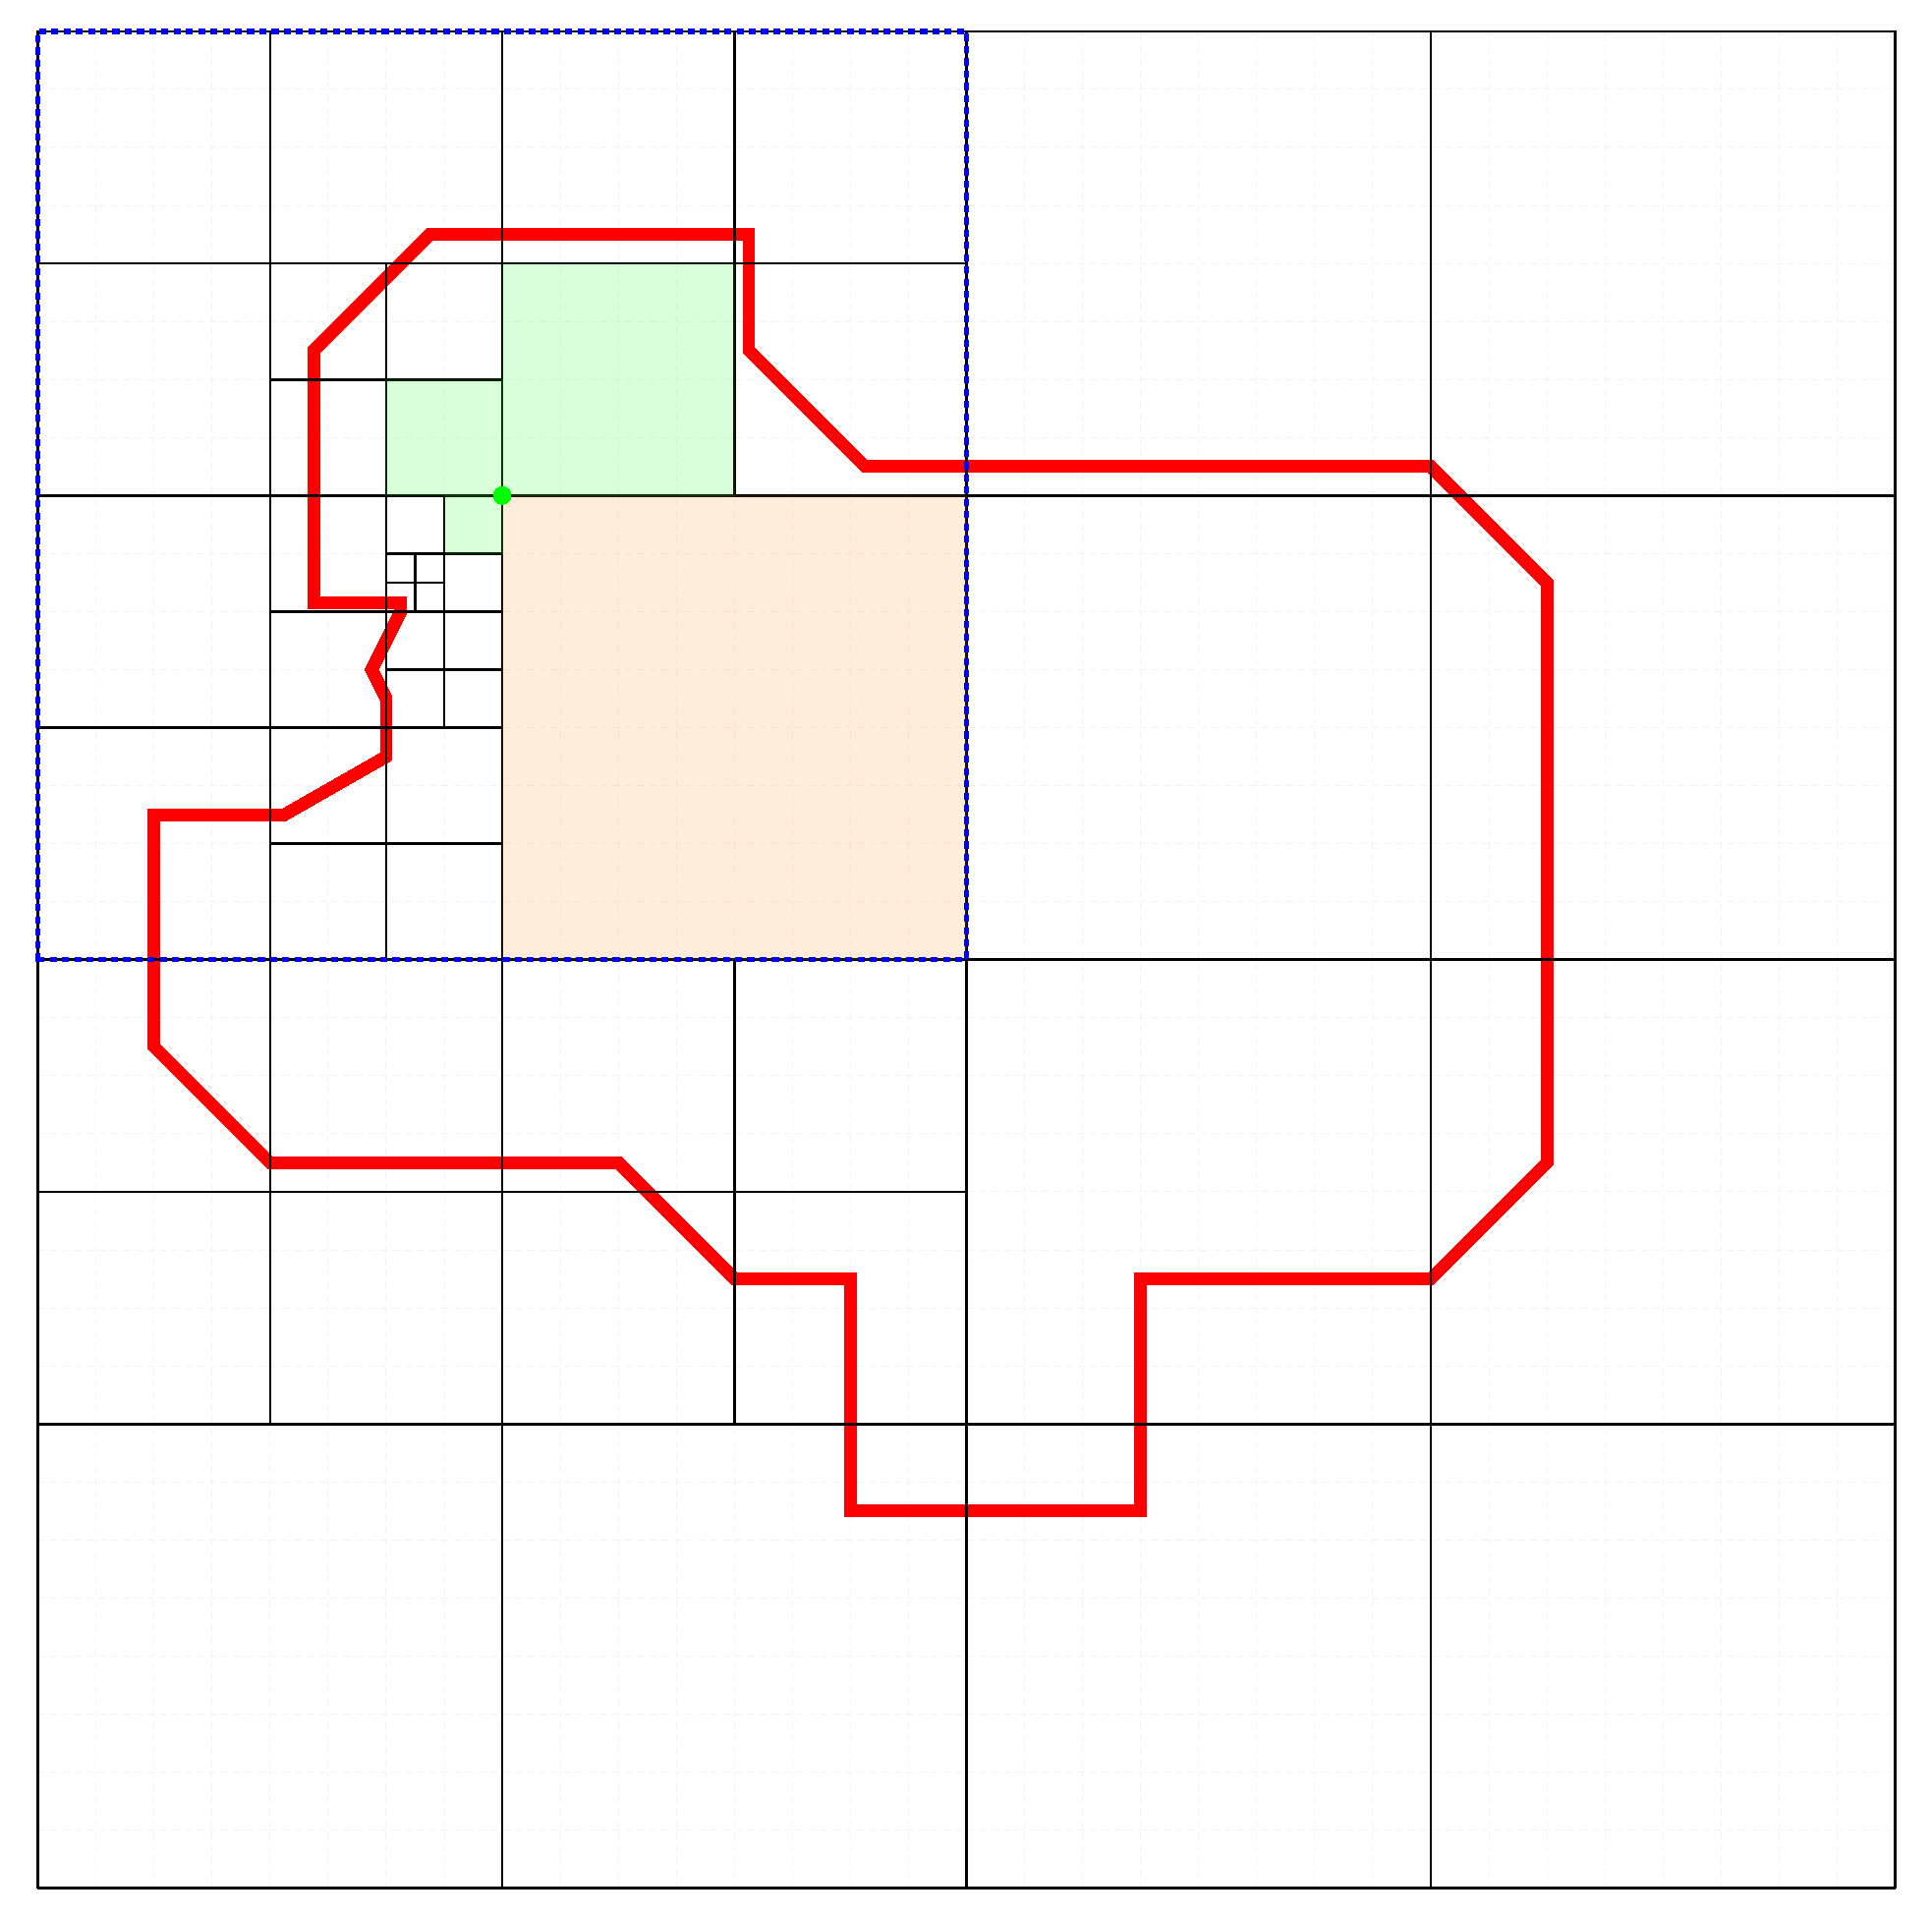
\includegraphics[page=1,width=0.6\textwidth]{figures/05-EmptyCells/Example}
\end{frame}
\begin{frame}{The Empty Cell problem...}
    \centering
	\includegraphics[page=2,width=0.6\textwidth]{figures/05-EmptyCells/Example}
\end{frame}
\begin{frame}{The Empty Cell problem...}
    \centering
	\includegraphics[page=3,width=0.6\textwidth]{figures/05-EmptyCells/Example}
\end{frame}

\begin{frame}{Correctness experiments...}
    \begin{enumerate}
        \item Run and extract polygons of the overlay operator from our implementation.
        \item Run and extract polygons of the overlay operator using QGIS.
        \item Run difference operator on the two outputs using QGIS.
        \item If outputs are equal, difference operator must be empty.
    \end{enumerate}
\end{frame}
\begin{frame}{Correctness experiments...}{Philadelphia districts 2000 (381 polygons) and 2010 (384 polygons)}
    \centering
	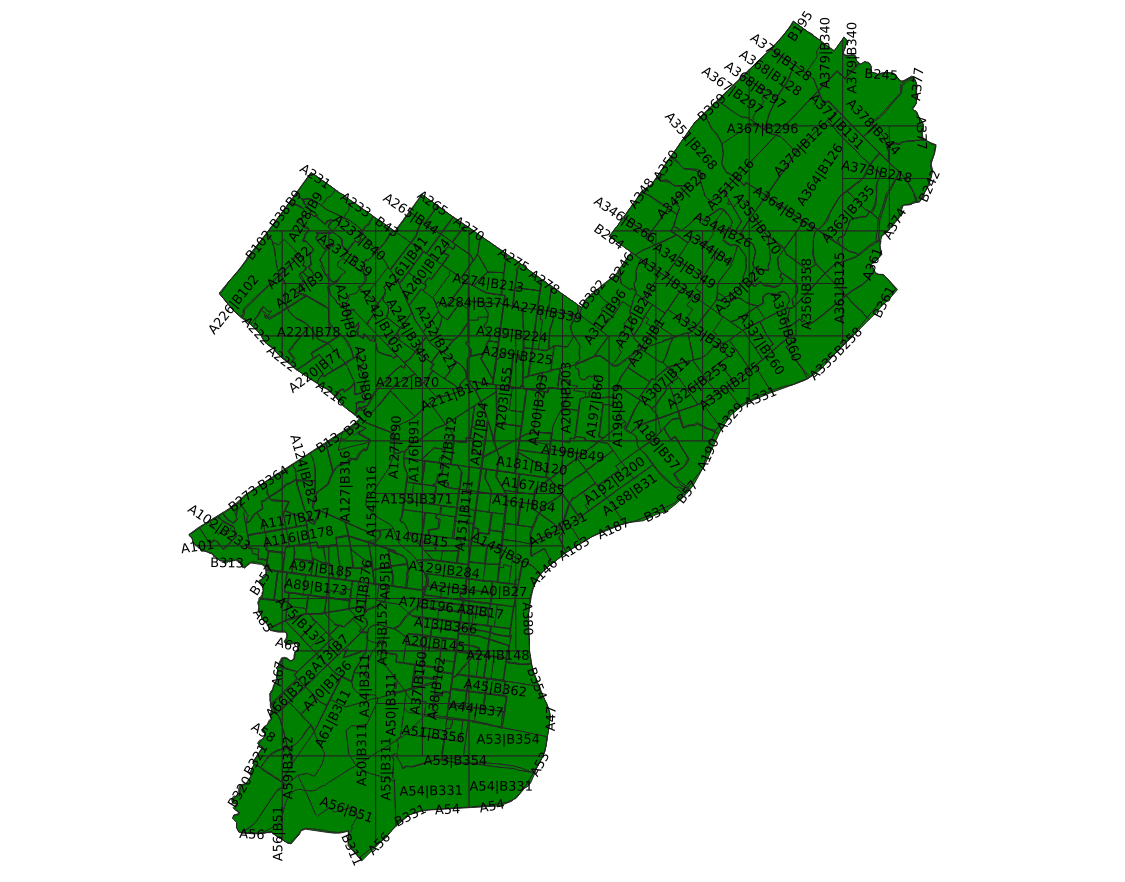
\includegraphics[trim=1cm 0 1cm 0, clip, width=0.7\textwidth]{figures/06-Correctness/Phili_Faces}
\end{frame}
\begin{frame}{Correctness experiments...}{Intersections...}
    \centering
	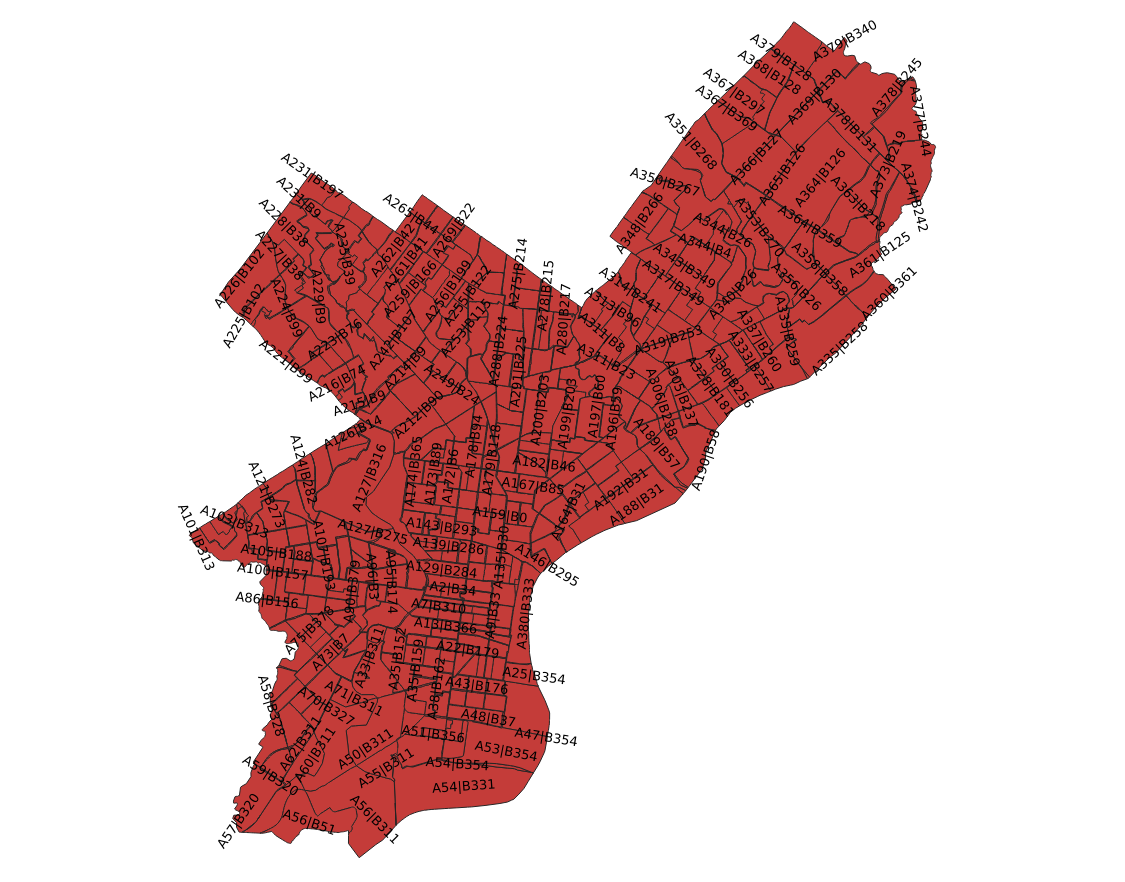
\includegraphics[trim=1cm 0 1cm 0, clip, width=0.7\textwidth]{figures/06-Correctness/Phili_Intersections}
\end{frame}
\begin{frame}{Correctness experiments...}{Symmetric difference...}
    \centering
	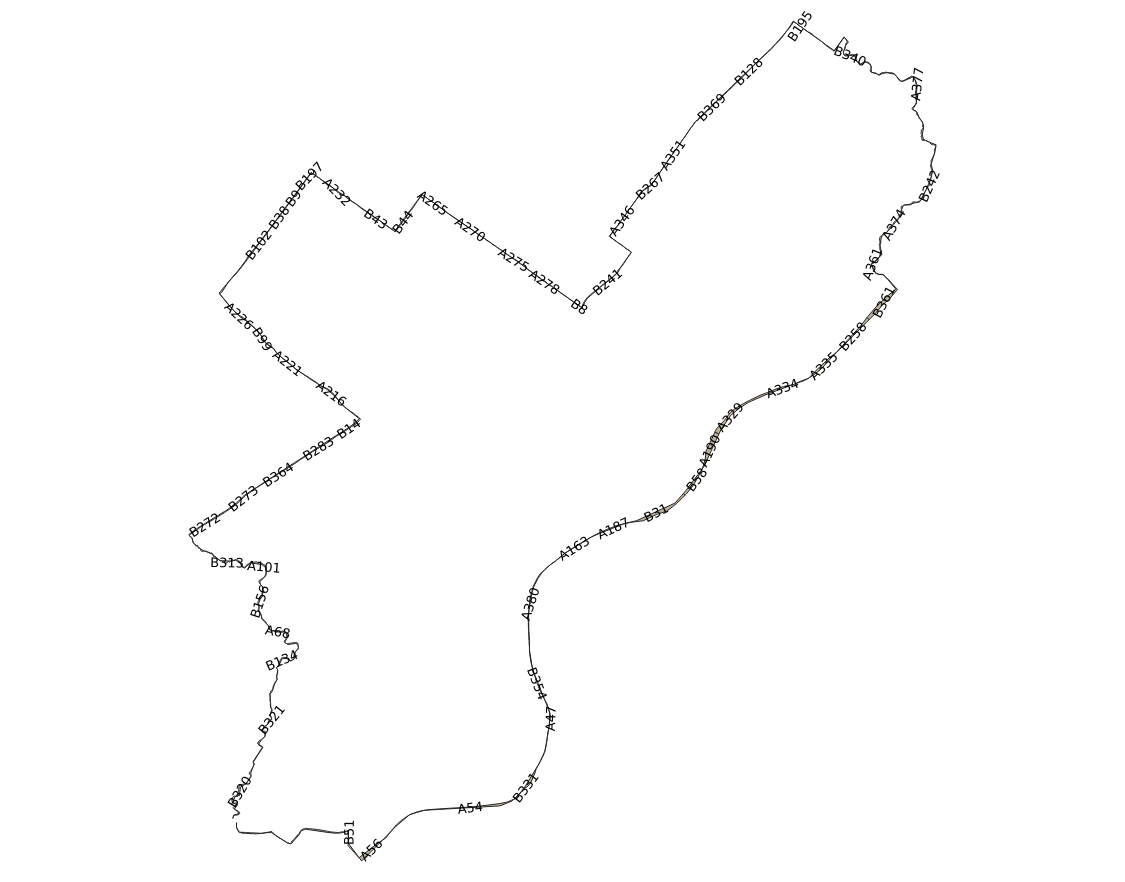
\includegraphics[trim=1cm 0 1cm 0, clip, width=0.7\textwidth]{figures/06-Correctness/Phili_Symmetric}
\end{frame}

\begin{frame}{Performance experiments...}{CA districts 2000 (7028 polygons) and 2010 (8047 polygons)}
    \centering
	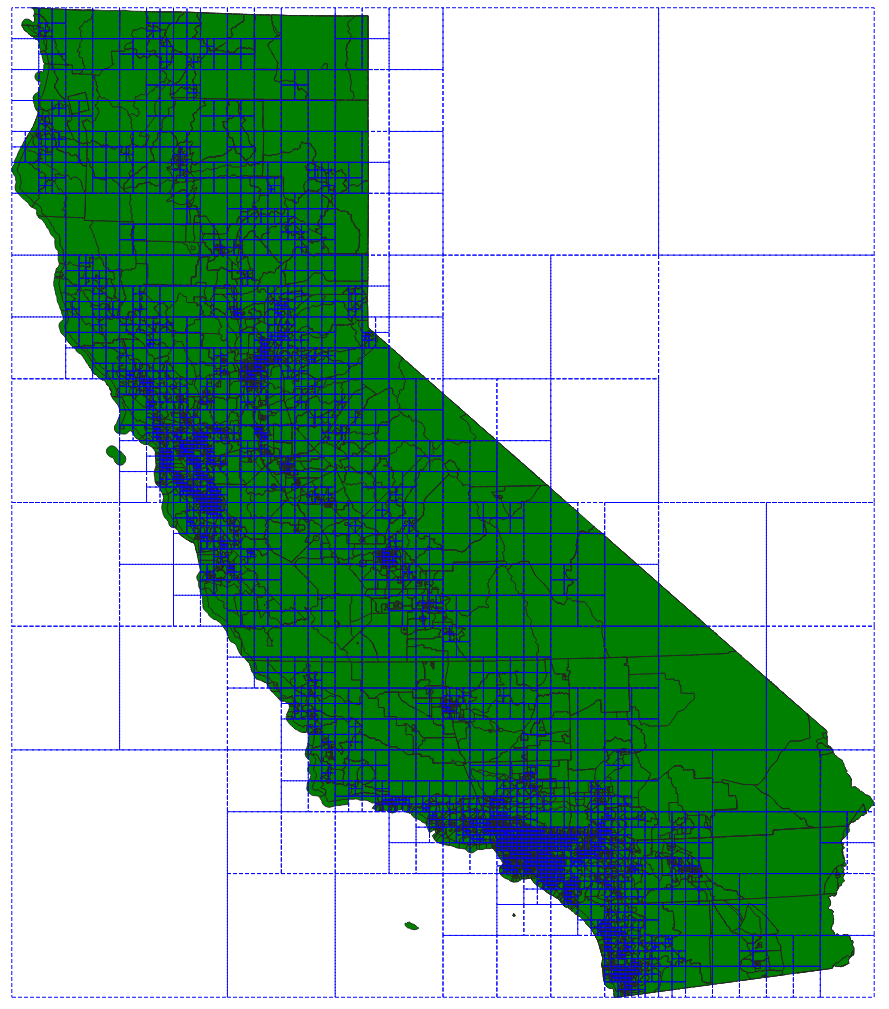
\includegraphics[trim=1cm 0 1cm 0, clip, width=0.5\textwidth]{figures/06-Correctness/CA_Faces}
\end{frame}

\begin{frame}{Performance experiments...}{Working on CGAL implementation}
    \begin{itemize}
        \item Based on Arrangements in 2D in the CGAL library (Section 8. Extending the DCEL))\footnote{\tiny \url{https://doc.cgal.org/latest/Arrangement_on_surface_2/index.html\#title51}}.
        \item Theory and resources are discussed at ``\textit{CGAL Arrangements and Their Applications: A Step-by-Step Guide}'' (Fogel et al, 2012)\footnote{\tiny \url{https://www.springer.com/gp/book/9783642172823}}.
        \item Code available at repository\footnote{\tiny \url{https://github.com/aocalderon/RIDIR/tree/master/Code/CGAL/DCEL}}.
        \item Performance is similar to previous work (Haran and Halperin, 2009\footnote{\tiny \url{https://dl.acm.org/doi/10.1145/1412228.1412237}}) and discussed with their authors.
    \end{itemize}
\end{frame}

\begin{frame}{Performance experiments...}
    \centering
    \begin{tabular}{ll}
        \hline
        \textbf{SDCEL} & \textbf{Execution time [s]} \\
        \hline
        Partitioning & 10.22 \\
        Building single DCELs & 4.02 \\
        Updating empy cells & 7.82 \\
        Merging DCELs & 9.62 \\
        \textbf{Total} & \textbf{31.69} \\
        \hline \\
        & \\
        \hline
        \textbf{CGAL} & \textbf{Execution time [s]} \\
        Building single DCELs & 594.01 \\
        Merging DCELs & 14.64 \\
        \textbf{Total} & \textbf{608.66} \\
        \hline
    \end{tabular} 
\end{frame}

\begin{frame}{What's next?}
    \begin{itemize}
        \item Currently working on Scale up and Speed up experiment tests.
        \item Exploring further case uses or expermients.
    \end{itemize}
\end{frame}

\end{document}
